The sensitivity of the signal regions proposed in Section~\ref{sec:sr} is evaluated with more refined statistical tools in this section, 
by using the HistFitter framework~\cite{HistFitter} to perform hypothesis tests for the different signal scenarios of interest. 
The event yields assumed in these test are the ones predicted by the set of Monte-Carlo samples described in section~\ref{sec:samples}, 
and the object selections detailed in Sections~\ref{sec:objects} and~\ref{sec:evtsel}. In all of the following, the fits use simple counting experiments,
i.e. no binning in any kinematic variable is considered. This choice was made in order to reduce the number of nuisance parameters in the fits.

\subsection{Non-combination of signal regions}

A set of dedicated studies has been performed to assess if, with an integrated luminosity between 2 and 3 fb$^{-1}$, a significant
extension of the reach of the analysis could be achieved by combining different signal regions.
For each of the four signal grid unders study, a ``golden'' signal region is selected as the one with the best expected performance. 
This is used as baseline result for each grid. In addition, an additional fit is also performed, where all signal regions are combined together.

The results of this study are reported in Figure \ref{fig:histfitter_combination}, where the signal region definitions in Table \ref{tab:SRdef2} have been used.
The fits are performed on MC only (i.e. blinding the data).
All experimental systematics are considered, and the only theory systematic included are the PDF error and a 30\% flat uncertainty on the background cross sections.
As shown in the plots, the gain from combining the signal regions is overall modest, and the decision was taken to perform simpler fits, i.e. without SR combination.

\begin{figure}[htb!]
\centering
\subfigure{\includegraphics[width=0.49\textwidth]{HISTFITTER/{exclusion2015SameSignMc15SusyGtt_nom_IntNote_2.47fb_V02_Excl_winter2015SameSign_output_hypotest__1_harvest_fix_list}.pdf}}
\subfigure{\includegraphics[width=0.49\textwidth]{HISTFITTER/{exclusion2015SameSignMc15SusyBtt_nom_IntNote_2.47fb_V02_Excl_winter2015SameSign_output_hypotest__1_harvest_fix_list}.pdf}}
\subfigure{\includegraphics[width=0.49\textwidth]{HISTFITTER/{exclusion2015SameSignMc15SusyGG2StepWZ_nom_IntNote_2.47fb_V02_Excl_winter2015SameSign_output_hypotest__1_harvest_fix_list}.pdf}}
\subfigure{\includegraphics[width=0.49\textwidth]{HISTFITTER/{exclusion2015SameSignMc15SusyGSL_nom_IntNote_2.47fb_V02_Excl_winter2015SameSign_output_hypotest__1_harvest_fix_list}.pdf}}
	
\caption{Comparison of the analysis sensitivities for different signal grids assuming 2.47~fb$^{-1}$.
The exclusion curve obtained combining all the signal regions is only marginally
better than the result obtained using only the best-performing signal region. Data is blinded in this plot.}
\label{fig:histfitter_combination}
\end{figure}
	



%\subsection{Impact of systematic errors}
%
%In order to verify that no individual systematic error is having a large impact on the performance of the analysis, a second set of blind fits has been perfrmed in which,
%together with the main result, the expected exclusion curves with different systematic uncertainties are considered.
%The combinations of systematic undertainties shown in the following are
%\begin{itemize}
% \item \textit{No systematics}: no systematic errors are considered
% \item \textit{Only experimental systematics}: this includes the systematics related to lepton/jet trigger/reconstruction/identification, as well as
% all the systematics on momentum/energy scales and resolutions.
% \item \textit{Experimental systematics with Fakes}: in addition to the experimental systematics, the systematic on the data-driven fake lepton background is also considered.
%  \item \textit{Experimental systematics with Fakes and Charge MisID}: in addition to the experimental systematics and the one on the data-driven fake lepton background,
%  the systematic on the data-driven charge mis-id background is added to the fit configuration.
%\end{itemize}
%
%
%Figure \ref{fig:histfitter_systematics} summarizes the results of these tests. The fits use the signal region definitions in Table \ref{tab:SRdef2},
%and are performed on MC only (i.e. blinding the data).
%As shown in the plots, the 
%
%\begin{figure}[htb!]
%\centering
%\subfigure{\includegraphics[width=0.49\textwidth]{HISTFITTER/{exclusion2015SameSignMc15SusyGtt_nom_IntNote_2.47fb_V10_Excl_winter2015SameSign_output_hypotest__1_harvest_fix_list}.pdf}}
%\subfigure{\includegraphics[width=0.49\textwidth]{HISTFITTER/{exclusion2015SameSignMc15SusyBtt_nom_IntNote_2.47fb_V10_Excl_winter2015SameSign_output_hypotest__1_harvest_fix_list}.pdf}}
%\subfigure{\includegraphics[width=0.49\textwidth]{HISTFITTER/{exclusion2015SameSignMc15SusyGG2StepWZ_nom_IntNote_2.47fb_V10_Excl_winter2015SameSign_output_hypotest__1_harvest_fix_list}.pdf}}
%\subfigure{\includegraphics[width=0.49\textwidth]{HISTFITTER/{exclusion2015SameSignMc15SusyGSL_nom_IntNote_2.47fb_V10_Excl_winter2015SameSign_output_hypotest__1_harvest_fix_list}.pdf}}
%
%\caption{Impact of the systematic errors on the performance of the analysis. The result with all systematics is compared to different combination of systematic errors. No single
%systematic appears to dominate the performance, with the exception of the sbottom 1-step decays, where the systematic due to fakes appears to modify significantly the
%of the expected exclusion.}
%\label{fig:histfitter_systematics}
%\end{figure}

\subsection{Background-only fits}

The following tables show the event yields for background-only fits with \textit{blinded} data. The purpose of these studies is to evaluate the overall consistency of
the fit setup and to have an idea of the impact of the systematic uncertainties on the fit results. Tables \ref{tab:histfitter:yields:bgonly:SR0b3j},
\ref{tab:histfitter:yields:bgonly:SR0b5j}, \ref{tab:histfitter:yields:bgonly:SR1b} and \ref{tab:histfitter:yields:bgonly:SR3b} show the event yields before and after the fits. 
These numbers are identical to the (condensed) ones presented in table~\ref{tab:sr_yields}. 
The systematic errors after the fits are reported in Tables \ref{tab:histfitter:syst:bgonly:SR0b3j}, \ref{tab:histfitter:syst:bgonly:SR0b5j}, \ref{tab:histfitter:syst:bgonly:SR1b}
and \ref{tab:histfitter:syst:bgonly:SR3b}

\begin{table}
\begin{center}
\setlength{\tabcolsep}{0.0pc}
{\small
%%
\begin{tabular*}{\textwidth}{@{\extracolsep{\fill}}lr}
\noalign{\smallskip}\hline\noalign{\smallskip}
\noalign{\smallskip}\hline\noalign{\smallskip}
{\bf Yields}           & SR0b3j              \\[-0.05cm]
\noalign{\smallskip}\hline\noalign{\smallskip}
%%
Observed events          & $1$                    \\
\noalign{\smallskip}\hline\noalign{\smallskip}
%%
Fitted bkg events         & $1.47 \pm 0.44$              \\
\noalign{\smallskip}\hline\noalign{\smallskip}
%%
        Fitted WWjj events         & $0.00 \pm 0.00$              \\
%%
        Fitted WZ events         & $1.20 \pm 0.40$              \\
%%
        Fitted ttZ events         & $0.10 \pm 0.04$              \\
%%
        Fitted ttW events         & $0.02 \pm 0.01$              \\
%%
        Fitted Rare events         & $0.14 \pm 0.08$              \\
%%
        Fitted OtherMultiBoson events         & $0.01 \pm 0.01$              \\
%%
        Fitted Fakes events         & $0.00 \pm 0.00$              \\
%%
        Fitted MisCharge events         & $0.00 \pm 0.00$              \\
%%     
 \noalign{\smallskip}\hline\noalign{\smallskip}
%%
MC exp. SM events              & $1.47$              \\
\noalign{\smallskip}\hline\noalign{\smallskip}
%%
        MC exp. WWjj events         & $0.00$              \\
%%
        MC exp. WZ events         & $1.20$              \\
%%
        MC exp. ttZ events         & $0.10$              \\
%%
        MC exp. ttW events         & $0.02$              \\
%%
        MC exp. Rare events         & $0.14$              \\
%%
        MC exp. OtherMultiBoson events         & $0.01$              \\
%%
        MC exp. Fakes events         & $0.00$              \\
%%
        MC exp. MisCharge events         & $0.00$              \\
%%     \\
\noalign{\smallskip}\hline\noalign{\smallskip}
\end{tabular*}
%%%
}

\end{center}

\caption{Event yields for a background-only blind fit for SR0b3j, at an integrated luminosity of 3.21 fb$^{-1}$. Only systematic uncertainties are displayed for the individual processes, but the uncertainty on the total background also includes the statistical component. }
\label{tab:histfitter:yields:bgonly:SR0b3j}
\end{table}


\begin{table}
\begin{center}
\setlength{\tabcolsep}{0.0pc}
{\small
%%
\begin{tabular*}{\textwidth}{@{\extracolsep{\fill}}lr}
\noalign{\smallskip}\hline\noalign{\smallskip}
{\bf Yields}           & SR0b5j              \\[-0.05cm]
\noalign{\smallskip}\hline\noalign{\smallskip}
%%
Observed events          & $0$                    \\
\noalign{\smallskip}\hline\noalign{\smallskip}
%%
Fitted bkg events         & $0.88 \pm 0.29$              \\
\noalign{\smallskip}\hline\noalign{\smallskip}
%%
        Fitted WWjj events         & $0.12 \pm 0.06$              \\
%%
        Fitted WZ events         & $0.49 \pm 0.20$              \\
%%
        Fitted ttZ events         & $0.05 \pm 0.03$              \\
%%
        Fitted ttW events         & $0.08 \pm 0.04$              \\
%%
        Fitted Rare events         & $0.07 \pm 0.05$              \\
%%
        Fitted OtherMultiBoson events         & $0.00_{-0.00}^{+0.04}$              \\
%%
        Fitted Fakes events         & $0.05_{-0.05}^{+0.06}$              \\
%%
        Fitted MisCharge events         & $0.02 \pm 0.01$              \\
%%     
 \noalign{\smallskip}\hline\noalign{\smallskip}
%%
MC exp. SM events              & $0.88$              \\
\noalign{\smallskip}\hline\noalign{\smallskip}
%%
        MC exp. WWjj events         & $0.12$              \\
%%
        MC exp. WZ events         & $0.49$              \\
%%
        MC exp. ttZ events         & $0.05$              \\
%%
        MC exp. ttW events         & $0.08$              \\
%%
        MC exp. Rare events         & $0.07$              \\
%%
        MC exp. OtherMultiBoson events         & $0.00$              \\
%%
        MC exp. Fakes events         & $0.05$              \\
%%
        MC exp. MisCharge events         & $0.02$              \\
%%     \\
\noalign{\smallskip}\hline\noalign{\smallskip}
\end{tabular*}
%%%
}

\end{center}
\caption{Event yields for a background-only blind fit for SR0b5j, at an integrated luminosity of 3.21 fb$^{-1}$. Only systematic uncertainties are displayed for the individual processes, but the uncertainty on the total background also includes the statistical component.}
\label{tab:histfitter:yields:bgonly:SR0b5j}
\end{table}
%


\begin{table}
\begin{center}
\setlength{\tabcolsep}{0.0pc}
{\small
%%
\begin{tabular*}{\textwidth}{@{\extracolsep{\fill}}lr}
\noalign{\smallskip}\hline\noalign{\smallskip}
{\bf Yields}           & SR1b              \\[-0.05cm]
\noalign{\smallskip}\hline\noalign{\smallskip}
%%
Observed events          & $4$                    \\
\noalign{\smallskip}\hline\noalign{\smallskip}
%%
Fitted bkg events         & $4.48 \pm 1.02$              \\
\noalign{\smallskip}\hline\noalign{\smallskip}
%%
        Fitted WWjj events         & $0.03 \pm 0.01$              \\
%%
        Fitted WZ events         & $0.18 \pm 0.09$              \\
%%
        Fitted ttZ events         & $0.92 \pm 0.31$              \\
%%
        Fitted ttW events         & $1.14 \pm 0.38$              \\
%%
        Fitted Rare events         & $0.81 \pm 0.42$              \\
%%
        Fitted OtherMultiBoson events         & $0.00_{-0.00}^{+0.00}$              \\
%%
        Fitted Fakes events         & $0.79 \pm 0.57$              \\
%%
        Fitted MisCharge events         & $0.60 \pm 0.09$              \\
%%     
 \noalign{\smallskip}\hline\noalign{\smallskip}
%%
MC exp. SM events              & $4.48$              \\
\noalign{\smallskip}\hline\noalign{\smallskip}
%%
        MC exp. WWjj events         & $0.03$              \\
%%
        MC exp. WZ events         & $0.18$              \\
%%
        MC exp. ttZ events         & $0.92$              \\
%%
        MC exp. ttW events         & $1.14$              \\
%%
        MC exp. Rare events         & $0.81$              \\
%%
        MC exp. OtherMultiBoson events         & $0.00$              \\
%%
        MC exp. Fakes events         & $0.79$              \\
%%
        MC exp. MisCharge events         & $0.60$              \\
%%     \\
\noalign{\smallskip}\hline\noalign{\smallskip}
\end{tabular*}
%%%
}
\end{center}
\caption{Event yields for a background-only blind fit for SR1b, at an integrated luminosity of 3.21 fb$^{-1}$. Only systematic uncertainties are displayed for the individual processes, but the uncertainty on the total background also includes the statistical component.}
\label{tab:histfitter:yields:bgonly:SR1b}

\end{table}



\begin{table}
\begin{center}
\setlength{\tabcolsep}{0.0pc}
{\small
%%
\begin{tabular*}{\textwidth}{@{\extracolsep{\fill}}lr}
\noalign{\smallskip}\hline\noalign{\smallskip}
{\bf Yields}           & SR3b              \\[-0.05cm]
\noalign{\smallskip}\hline\noalign{\smallskip}
{\bf Yields}           & SR3b              \\[-0.05cm]
\noalign{\smallskip}\hline\noalign{\smallskip}
%%
Observed events          & $0$                    \\
\noalign{\smallskip}\hline\noalign{\smallskip}
%%
Fitted bkg events         & $0.80 \pm 0.25$              \\
\noalign{\smallskip}\hline\noalign{\smallskip}
%%
        Fitted WWjj events         & $0.00 \pm 0.00$              \\
%%
        Fitted WZ events         & $0.00 \pm 0.00$              \\
%%
        Fitted ttZ events         & $0.14 \pm 0.06$              \\
%%
        Fitted ttW events         & $0.10 \pm 0.05$              \\
%%
        Fitted Rare events         & $0.24 \pm 0.14$              \\
%%
        Fitted OtherMultiBoson events         & $0.00 \pm 0.00$              \\
%%
        Fitted Fakes events         & $0.13 \pm 0.09$              \\
%%
        Fitted MisCharge events         & $0.19 \pm 0.04$              \\
%%     
 \noalign{\smallskip}\hline\noalign{\smallskip}
%%
MC exp. SM events              & $0.80$              \\
\noalign{\smallskip}\hline\noalign{\smallskip}
%%
        MC exp. WWjj events         & $0.00$              \\
%%
        MC exp. WZ events         & $0.00$              \\
%%
        MC exp. ttZ events         & $0.14$              \\
%%
        MC exp. ttW events         & $0.10$              \\
%%
        MC exp. Rare events         & $0.24$              \\
%%
        MC exp. OtherMultiBoson events         & $0.00$              \\
%%
        MC exp. Fakes events         & $0.13$              \\
%%
        MC exp. MisCharge events         & $0.19$              \\
%%     \\
\noalign{\smallskip}\hline\noalign{\smallskip}
\end{tabular*}
%%%
}
\end{center}
\caption{Event yields for a background-only blind fit for SR3b, at an integrated luminosity of 3.21 fb$^{-1}$. Only systematic uncertainties are displayed for the individual processes, but the uncertainty on the total background also includes the statistical component.}
\label{tab:histfitter:yields:bgonly:SR3b}
\end{table}
%



\begin{table}
\begin{center}
\setlength{\tabcolsep}{0.0pc}
\begin{tabular*}{\textwidth}{@{\extracolsep{\fill}}lc}
\noalign{\smallskip}\hline\noalign{\smallskip}
{\bf Uncertainty of channel}                                    & SR0b3j            \\
\noalign{\smallskip}\hline\noalign{\smallskip}
%%
Total background expectation             &  $1.47$       \\
%% \\
\noalign{\smallskip}\hline\noalign{\smallskip}
%%
Total statistical $(\sqrt{N_{\rm exp}})$              & $\pm 1.21$       \\
%%
Total background systematic               & $\pm 0.44\ [29.65\%] $             \\
\noalign{\smallskip}\hline\noalign{\smallskip}
\noalign{\smallskip}\hline\noalign{\smallskip}
%%
alpha\_theoryUncertWZ\_SR0b3j         & $\pm 0.34$       \\
%%
alpha\_JET\_scale\_NP1         & $\pm 0.17$       \\
%%
gamma\_stat\_SR0b3j\_cuts\_bin\_0         & $\pm 0.16$       \\
%%
alpha\_PDF         & $\pm 0.09$       \\
%%
Lumi         & $\pm 0.07$       \\
%%
alpha\_theoryUncertRare         & $\pm 0.07$       \\
%%
alpha\_pileupBKG         & $\pm 0.07$       \\
%%
alpha\_FT\_B         & $\pm 0.06$       \\
%%
alpha\_JET\_scale\_NP2         & $\pm 0.05$       \\
%%
alpha\_JET\_reso         & $\pm 0.04$       \\
%%
alpha\_JET\_scale\_NP3         & $\pm 0.04$       \\
%%
alpha\_theoryUncertTTbarV\_SR0b3j         & $\pm 0.04$       \\
%%
alpha\_elID         & $\pm 0.02$       \\
%%
alpha\_MET\_Soft\_reso\_Para         & $\pm 0.02$       \\
%%
alpha\_muSys         & $\pm 0.02$       \\
%%
alpha\_FT\_Light         & $\pm 0.01$       \\
%%
alpha\_FT\_C         & $\pm 0.01$       \\
%%
alpha\_muIsoSys         & $\pm 0.01$       \\
%%
alpha\_elReco         & $\pm 0.01$       \\
%%
alpha\_Mu\_ID         & $\pm 0.01$       \\
%%
alpha\_MET\_Soft\_Scale         & $\pm 0.01$       \\
%%
alpha\_muStat         & $\pm 0.01$       \\
%%
alpha\_FT\_Extra1         & $\pm 0.00$       \\
%%
alpha\_theoryUncertOtherMB         & $\pm 0.00$       \\
%%
alpha\_muIsoStat         & $\pm 0.00$       \\
%%
alpha\_EG\_Resolution         & $\pm 0.00$       \\
%%
alpha\_MET\_Soft\_reso\_Perp         & $\pm 0.00$       \\
%%
alpha\_Mu\_MS         & $\pm 0.00$       \\
%%
alpha\_elTrig         & $\pm 0.00$       \\
%%
alpha\_FT\_Extra2         & $\pm 0.00$       \\
%%
alpha\_Mu\_Scale         & $\pm 0.00$       \\
%%
alpha\_EG\_Scale         & $\pm 0.00$       \\
%%
alpha\_JET\_AFII         & $\pm 0.00$       \\
%%
\noalign{\smallskip}\hline\noalign{\smallskip}
\end{tabular*}
\end{center}
\caption{Systematics for a background-only blind fit in SR0b3j, at an integrated luminosity of 3.21 fb$^{-1}$.}
\label{tab:histfitter:syst:bgonly:SR0b3j}
\end{table}
%


\begin{table}
\begin{center}
\setlength{\tabcolsep}{0.0pc}
\begin{tabular*}{\textwidth}{@{\extracolsep{\fill}}lc}
\noalign{\smallskip}\hline\noalign{\smallskip}
{\bf Uncertainty of channel}                                    & SR0b5j            \\
\noalign{\smallskip}\hline\noalign{\smallskip}
%%
Total background expectation             &  $0.88$       \\
%% \\
\noalign{\smallskip}\hline\noalign{\smallskip}
%%
Total statistical $(\sqrt{N_{\rm exp}})$              & $\pm 0.94$       \\
%%
Total background systematic               & $\pm 0.29\ [33.52\%] $             \\
\noalign{\smallskip}\hline\noalign{\smallskip}
\noalign{\smallskip}\hline\noalign{\smallskip}
%%
gamma\_stat\_SR0b5j\_cuts\_bin\_0         & $\pm 0.20$       \\
%%
alpha\_theoryUncertWZ\_SR0b5j         & $\pm 0.14$       \\
%%
alpha\_JET\_reso         & $\pm 0.08$       \\
%%
alpha\_pileupBKG         & $\pm 0.06$       \\
%%
alpha\_FT\_B         & $\pm 0.06$       \\
%%
alpha\_PDF         & $\pm 0.06$       \\
%%
alpha\_JET\_scale\_NP1         & $\pm 0.06$       \\
%%
alpha\_JET\_scale\_NP3         & $\pm 0.06$       \\
%%
alpha\_syst\_fake\_SR0b5j         & $\pm 0.06$       \\
%%
alpha\_JET\_scale\_NP2         & $\pm 0.05$       \\
%%
Lumi         & $\pm 0.04$       \\
%%
alpha\_theoryUncertTTbarV\_SR0b5j         & $\pm 0.04$       \\
%%
alpha\_theoryUncertWWjj\_SR0b5j         & $\pm 0.04$       \\
%%
alpha\_theoryUncertRare         & $\pm 0.03$       \\
%%
alpha\_Mu\_MS         & $\pm 0.02$       \\
%%
alpha\_MET\_Soft\_reso\_Perp         & $\pm 0.01$       \\
%%
alpha\_FT\_C         & $\pm 0.01$       \\
%%
alpha\_elID         & $\pm 0.01$       \\
%%
alpha\_FT\_Light         & $\pm 0.01$       \\
%%
alpha\_MET\_Soft\_Scale         & $\pm 0.01$       \\
%%
alpha\_muSys         & $\pm 0.01$       \\
%%
alpha\_muIsoSys         & $\pm 0.00$       \\
%%
alpha\_elReco         & $\pm 0.00$       \\
%%
alpha\_FT\_Extra1         & $\pm 0.00$       \\
%%
alpha\_syst\_misch\_SR0b5j         & $\pm 0.00$       \\
%%
alpha\_elTrig         & $\pm 0.00$       \\
%%
alpha\_muStat         & $\pm 0.00$       \\
%%
alpha\_FT\_Extra2         & $\pm 0.00$       \\
%%
alpha\_MET\_Soft\_reso\_Para         & $\pm 0.00$       \\
%%
alpha\_muIsoStat         & $\pm 0.00$       \\
%%
alpha\_EG\_Scale         & $\pm 0.00$       \\
%%
alpha\_Mu\_ID         & $\pm 0.00$       \\
%%
alpha\_Mu\_Scale         & $\pm 0.00$       \\
%%
alpha\_theoryUncertOtherMB         & $\pm 0.00$       \\
%%
alpha\_EG\_Resolution         & $\pm 0.00$       \\
%%
alpha\_JET\_AFII         & $\pm 0.00$       \\
%%
\noalign{\smallskip}\hline\noalign{\smallskip}
\end{tabular*}
\end{center}
\caption{Systematics for a background-only blind fit in SR0b5j, at an integrated luminosity of 3.21 fb$^{-1}$.}
\label{tab:histfitter:syst:bgonly:SR0b5j}
\end{table}
%



\begin{table}
\begin{center}
\setlength{\tabcolsep}{0.0pc}
\begin{tabular*}{\textwidth}{@{\extracolsep{\fill}}lc}
\noalign{\smallskip}\hline\noalign{\smallskip}
{\bf Uncertainty of channel}                                    & SR1b            \\
\noalign{\smallskip}\hline\noalign{\smallskip}
%%
Total background expectation             &  $4.48$       \\
%% \\
\noalign{\smallskip}\hline\noalign{\smallskip}
%%
Total statistical $(\sqrt{N_{\rm exp}})$              & $\pm 2.12$       \\
%%
Total background systematic               & $\pm 1.02\ [22.83\%] $             \\
\noalign{\smallskip}\hline\noalign{\smallskip}
\noalign{\smallskip}\hline\noalign{\smallskip}
%%
alpha\_theoryUncertTTbarV\_SR1b         & $\pm 0.59$       \\
%%
alpha\_syst\_fake\_SR1b         & $\pm 0.56$       \\
%%
gamma\_stat\_SR1b\_cuts\_bin\_0         & $\pm 0.52$       \\
%%
alpha\_theoryUncertRare         & $\pm 0.40$       \\
%%
alpha\_PDF         & $\pm 0.29$       \\
%%
alpha\_JET\_scale\_NP1         & $\pm 0.25$       \\
%%
Lumi         & $\pm 0.15$       \\
%%
alpha\_FT\_B         & $\pm 0.13$       \\
%%
alpha\_JET\_scale\_NP2         & $\pm 0.12$       \\
%%
alpha\_JET\_reso         & $\pm 0.09$       \\
%%
alpha\_pileupBKG         & $\pm 0.07$       \\
%%
alpha\_JET\_scale\_NP3         & $\pm 0.06$       \\
%%
alpha\_theoryUncertWZ\_SR1b         & $\pm 0.05$       \\
%%
alpha\_syst\_misch\_SR1b         & $\pm 0.05$       \\
%%
alpha\_FT\_C         & $\pm 0.04$       \\
%%
alpha\_elID         & $\pm 0.04$       \\
%%
alpha\_MET\_Soft\_reso\_Para         & $\pm 0.03$       \\
%%
alpha\_muSys         & $\pm 0.02$       \\
%%
alpha\_elReco         & $\pm 0.02$       \\
%%
alpha\_muIsoSys         & $\pm 0.01$       \\
%%
alpha\_MET\_Soft\_Scale         & $\pm 0.01$       \\
%%
alpha\_FT\_Extra1         & $\pm 0.01$       \\
%%
alpha\_Mu\_MS         & $\pm 0.01$       \\
%%
alpha\_theoryUncertWWjj\_SR1b         & $\pm 0.01$       \\
%%
alpha\_elTrig         & $\pm 0.01$       \\
%%
alpha\_Mu\_ID         & $\pm 0.01$       \\
%%
alpha\_muStat         & $\pm 0.01$       \\
%%
alpha\_MET\_Soft\_reso\_Perp         & $\pm 0.01$       \\
%%
alpha\_Mu\_Scale         & $\pm 0.00$       \\
%%
alpha\_EG\_Resolution         & $\pm 0.00$       \\
%%
alpha\_muIsoStat         & $\pm 0.00$       \\
%%
alpha\_EG\_Scale         & $\pm 0.00$       \\
%%
alpha\_JET\_AFII         & $\pm 0.00$       \\
%%
alpha\_FT\_Extra2         & $\pm 0.00$       \\
%%
alpha\_FT\_Light         & $\pm 0.00$       \\
%%
alpha\_theoryUncertOtherMB         & $\pm 0.00$       \\
%%
\noalign{\smallskip}\hline\noalign{\smallskip}
\end{tabular*}
\end{center}
\caption{Systematics for a background-only blind fit in SR1b, at an integrated luminosity of 3.21 fb$^{-1}$.}
\label{tab:histfitter:syst:bgonly:SR1b}
\end{table}
%



\begin{table}
\begin{center}
\setlength{\tabcolsep}{0.0pc}
\begin{tabular*}{\textwidth}{@{\extracolsep{\fill}}lc}
\noalign{\smallskip}\hline\noalign{\smallskip}
{\bf Uncertainty of channel}                                    & SR3b            \\
\noalign{\smallskip}\hline\noalign{\smallskip}
%%
Total background expectation             &  $0.80$       \\
%% \\
\noalign{\smallskip}\hline\noalign{\smallskip}
%%
Total statistical $(\sqrt{N_{\rm exp}})$              & $\pm 0.90$       \\
%%
Total background systematic               & $\pm 0.25\ [30.66\%] $             \\
\noalign{\smallskip}\hline\noalign{\smallskip}
\noalign{\smallskip}\hline\noalign{\smallskip}
%%
gamma\_stat\_SR3b\_cuts\_bin\_0         & $\pm 0.16$       \\
%%
alpha\_theoryUncertRare         & $\pm 0.12$       \\
%%
alpha\_syst\_fake\_SR3b         & $\pm 0.09$       \\
%%
alpha\_theoryUncertTTbarV\_SR3b         & $\pm 0.07$       \\
%%
alpha\_FT\_B         & $\pm 0.07$       \\
%%
alpha\_PDF         & $\pm 0.06$       \\
%%
alpha\_FT\_C         & $\pm 0.04$       \\
%%
alpha\_JET\_scale\_NP1         & $\pm 0.03$       \\
%%
Lumi         & $\pm 0.02$       \\
%%
alpha\_FT\_Light         & $\pm 0.02$       \\
%%
alpha\_syst\_misch\_SR3b         & $\pm 0.02$       \\
%%
alpha\_JET\_reso         & $\pm 0.02$       \\
%%
alpha\_JET\_scale\_NP2         & $\pm 0.02$       \\
%%
alpha\_pileupBKG         & $\pm 0.01$       \\
%%
alpha\_elID         & $\pm 0.01$       \\
%%
alpha\_MET\_Soft\_reso\_Perp         & $\pm 0.01$       \\
%%
alpha\_FT\_Extra1         & $\pm 0.01$       \\
%%
alpha\_MET\_Soft\_reso\_Para         & $\pm 0.00$       \\
%%
alpha\_Mu\_MS         & $\pm 0.00$       \\
%%
alpha\_FT\_Extra2         & $\pm 0.00$       \\
%%
alpha\_muSys         & $\pm 0.00$       \\
%%
alpha\_elReco         & $\pm 0.00$       \\
%%
alpha\_JET\_scale\_NP3         & $\pm 0.00$       \\
%%
alpha\_muIsoSys         & $\pm 0.00$       \\
%%
alpha\_MET\_Soft\_Scale         & $\pm 0.00$       \\
%%
alpha\_EG\_Resolution         & $\pm 0.00$       \\
%%
alpha\_elTrig         & $\pm 0.00$       \\
%%
alpha\_muStat         & $\pm 0.00$       \\
%%
alpha\_EG\_Scale         & $\pm 0.00$       \\
%%
alpha\_muIsoStat         & $\pm 0.00$       \\
%%
alpha\_JET\_AFII         & $\pm 0.00$       \\
%%
alpha\_Mu\_ID         & $\pm 0.00$       \\
%%
alpha\_Mu\_Scale         & $\pm 0.00$       \\
%%
\noalign{\smallskip}\hline\noalign{\smallskip}
\end{tabular*}
\end{center}
\caption{Systematics for a background-only blind fit in SR3b, at an integrated luminosity of 3.2 fb$^{-1}$.}
\label{tab:histfitter:syst:bgonly:SR3b}
\end{table}
%

\subsection{Discovery fits}
A first estimate of the level of agreement between data and MC can be obtained using \textit{discovery} fits. 
These are model-independent discovery fits in which an extra contribution is added to the SM backgrounds and a fit to data in the signal regions is performed. 
The result of the fit is the ``signal-strength'' of the additional contribution. 
The resulting event yields are shown in Tables \ref{tab:histfitter:yields:disc:SR0b3j}, \ref{tab:histfitter:yields:disc:SR0b5j}, 
\ref{tab:histfitter:yields:disc:SR1b} and \ref{tab:histfitter:yields:disc:SR3b}.

\begin{table}
\begin{center}
\setlength{\tabcolsep}{0.0pc}
{\small
%%
\begin{tabular*}{\textwidth}{@{\extracolsep{\fill}}lr}
\noalign{\smallskip}\hline\noalign{\smallskip}
{\bf Yields}           & SR0b3j              \\[-0.05cm]
\noalign{\smallskip}\hline\noalign{\smallskip}
%%
Observed events          & $3$                    \\
\noalign{\smallskip}\hline\noalign{\smallskip}
%%
Fitted bkg events         & $3.01 \pm 1.61$              \\
\noalign{\smallskip}\hline\noalign{\smallskip}
%%
        Fitted WWjj events         & $0.00 \pm 0.00$              \\
%%
        Fitted WZ events         & $1.20 \pm 0.43$              \\
%%
        Fitted ttZ events         & $0.10 \pm 0.04$              \\
%%
        Fitted ttW events         & $0.02 \pm 0.01$              \\
%%
        Fitted Rare events         & $0.14 \pm 0.08$              \\
%%
        Fitted OtherMultiBoson events         & $0.01 \pm 0.01$              \\
%%
        Fitted DiscoveryMode\_SR0b3j events         & $1.54_{-1.54}^{+1.66}$              \\
%%
        Fitted Fakes events         & $0.00 \pm 0.00$              \\
%%
        Fitted MisCharge events         & $0.00 \pm 0.00$              \\
%%     
 \noalign{\smallskip}\hline\noalign{\smallskip}
%%
MC exp. SM events              & $2.47$              \\
\noalign{\smallskip}\hline\noalign{\smallskip}
%%
        MC exp. WWjj events         & $0.00$              \\
%%
        MC exp. WZ events         & $1.20$              \\
%%
        MC exp. ttZ events         & $0.10$              \\
%%
        MC exp. ttW events         & $0.02$              \\
%%
        MC exp. Rare events         & $0.14$              \\
%%
        MC exp. OtherMultiBoson events         & $0.01$              \\
%%
        MC exp. DiscoveryMode\_SR0b3j events         & $1.00$              \\
%%
        MC exp. Fakes events         & $0.00$              \\
%%
        MC exp. MisCharge events         & $0.00$              \\
%%     \\
\noalign{\smallskip}\hline\noalign{\smallskip}
\end{tabular*}
%%%
}
\end{center}
\caption{Event yields for a discovery fit SR0b3j, at an integrated luminosity of 3.21 fb$^{-1}$. Only systematic uncertainties are displayed for the individual processes, but the uncertainty on the total background also includes the statistical component.}
\label{tab:histfitter:yields:disc:SR0b3j}
\end{table}
%

\begin{table}
\begin{center}
\setlength{\tabcolsep}{0.0pc}
{\small
%%
\begin{tabular*}{\textwidth}{@{\extracolsep{\fill}}lr}
\noalign{\smallskip}\hline\noalign{\smallskip}
{\bf Yields}           & SR0b5j              \\[-0.05cm]
\noalign{\smallskip}\hline\noalign{\smallskip}
%%
Observed events          & $3$                    \\
\noalign{\smallskip}\hline\noalign{\smallskip}
%%
Fitted bkg events         & $3.02 \pm 1.73$              \\
\noalign{\smallskip}\hline\noalign{\smallskip}
%%
        Fitted WWjj events         & $0.12 \pm 0.06$              \\
%%
        Fitted WZ events         & $0.49 \pm 0.21$              \\
%%
        Fitted ttZ events         & $0.05 \pm 0.03$              \\
%%
        Fitted ttW events         & $0.08 \pm 0.04$              \\
%%
        Fitted Rare events         & $0.07 \pm 0.05$              \\
%%
        Fitted OtherMultiBoson events         & $0.00_{-0.00}^{+0.04}$              \\
%%
        Fitted DiscoveryMode\_SR0b5j events         & $2.14 \pm 1.76$              \\
%%
        Fitted Fakes events         & $0.05_{-0.05}^{+0.06}$              \\
%%
        Fitted MisCharge events         & $0.02 \pm 0.01$              \\
%%     
 \noalign{\smallskip}\hline\noalign{\smallskip}
%%
MC exp. SM events              & $1.88$              \\
\noalign{\smallskip}\hline\noalign{\smallskip}
%%
        MC exp. WWjj events         & $0.12$              \\
%%
        MC exp. WZ events         & $0.49$              \\
%%
        MC exp. ttZ events         & $0.05$              \\
%%
        MC exp. ttW events         & $0.08$              \\
%%
        MC exp. Rare events         & $0.07$              \\
%%
        MC exp. OtherMultiBoson events         & $0.00$              \\
%%
        MC exp. DiscoveryMode\_SR0b5j events         & $1.00$              \\
%%
        MC exp. Fakes events         & $0.05$              \\
%%
        MC exp. MisCharge events         & $0.02$              \\
%%     \\
\noalign{\smallskip}\hline\noalign{\smallskip}
\end{tabular*}
%%%
}
\end{center}
\caption{Event yields for a discovery fit SR0b5j, at an integrated luminosity of 3.21 fb$^{-1}$. Only systematic uncertainties are displayed for the individual processes, but the uncertainty on the total background also includes the statistical component.}
\label{tab:histfitter:yields:disc:SR0b5j}
\end{table}
%

\begin{table}
\begin{center}
\setlength{\tabcolsep}{0.0pc}
{\small
%%
\begin{tabular*}{\textwidth}{@{\extracolsep{\fill}}lr}
\noalign{\smallskip}\hline\noalign{\smallskip}
{\bf Yields}           & SR1b              \\[-0.05cm]
\noalign{\smallskip}\hline\noalign{\smallskip}
%%
Observed events          & $7$                    \\
\noalign{\smallskip}\hline\noalign{\smallskip}
%%
Fitted bkg events         & $7.03 \pm 2.46$              \\
\noalign{\smallskip}\hline\noalign{\smallskip}
%%
        Fitted WWjj events         & $0.03 \pm 0.01$              \\
%%
        Fitted WZ events         & $0.18 \pm 0.09$              \\
%%
        Fitted ttZ events         & $0.93 \pm 0.34$              \\
%%
        Fitted ttW events         & $1.15 \pm 0.41$              \\
%%
        Fitted Rare events         & $0.82 \pm 0.44$              \\
%%
        Fitted OtherMultiBoson events         & $0.00_{-0.00}^{+0.00}$              \\
%%
        Fitted DiscoveryMode\_SR1b events         & $2.51_{-2.51}^{+2.70}$              \\
%%
        Fitted Fakes events         & $0.81 \pm 0.60$              \\
%%
        Fitted MisCharge events         & $0.60 \pm 0.09$              \\
%%     
 \noalign{\smallskip}\hline\noalign{\smallskip}
%%
MC exp. SM events              & $5.48$              \\
\noalign{\smallskip}\hline\noalign{\smallskip}
%%
        MC exp. WWjj events         & $0.03$              \\
%%
        MC exp. WZ events         & $0.18$              \\
%%
        MC exp. ttZ events         & $0.92$              \\
%%
        MC exp. ttW events         & $1.14$              \\
%%
        MC exp. Rare events         & $0.81$              \\
%%
        MC exp. OtherMultiBoson events         & $0.00$              \\
%%
        MC exp. DiscoveryMode\_SR1b events         & $1.00$              \\
%%
        MC exp. Fakes events         & $0.79$              \\
%%
        MC exp. MisCharge events         & $0.60$              \\
%%     \\
\noalign{\smallskip}\hline\noalign{\smallskip}
\end{tabular*}
%%%
}
\end{center}
\caption{Event yields for a discovery fit SR1b, at an integrated luminosity of 3.21 fb$^{-1}$. Only systematic uncertainties are displayed for the individual processes, but the uncertainty on the total background also includes the statistical component.}
\label{tab:histfitter:yields:disc:SR1b}
\end{table}
%

\begin{table}
\begin{center}
\setlength{\tabcolsep}{0.0pc}
{\small
%%
\begin{tabular*}{\textwidth}{@{\extracolsep{\fill}}lr}
\noalign{\smallskip}\hline\noalign{\smallskip}
{\bf Yields}           & SR3b              \\[-0.05cm]
\noalign{\smallskip}\hline\noalign{\smallskip}
%%
Observed events          & $1$                    \\
\noalign{\smallskip}\hline\noalign{\smallskip}
%%
Fitted bkg events         & $1.04 \pm 0.67$              \\
\noalign{\smallskip}\hline\noalign{\smallskip}
%%
        Fitted WWjj events         & $0.00 \pm 0.00$              \\
%%
        Fitted WZ events         & $0.00 \pm 0.00$              \\
%%
        Fitted ttZ events         & $0.14 \pm 0.06$              \\
%%
        Fitted ttW events         & $0.10 \pm 0.05$              \\
%%
        Fitted Rare events         & $0.24 \pm 0.14$              \\
%%
        Fitted OtherMultiBoson events         & $0.00 \pm 0.00$              \\
%%
        Fitted DiscoveryMode\_SR3b events         & $0.23_{-0.23}^{+0.68}$              \\
%%
        Fitted Fakes events         & $0.13 \pm 0.09$              \\
%%
        Fitted MisCharge events         & $0.19 \pm 0.04$              \\
%%     
 \noalign{\smallskip}\hline\noalign{\smallskip}
%%
MC exp. SM events              & $1.80$              \\
\noalign{\smallskip}\hline\noalign{\smallskip}
%%
        MC exp. WWjj events         & $0.00$              \\
%%
        MC exp. WZ events         & $0.00$              \\
%%
        MC exp. ttZ events         & $0.14$              \\
%%
        MC exp. ttW events         & $0.10$              \\
%%
        MC exp. Rare events         & $0.24$              \\
%%
        MC exp. OtherMultiBoson events         & $0.00$              \\
%%
        MC exp. DiscoveryMode\_SR3b events         & $1.00$              \\
%%
        MC exp. Fakes events         & $0.13$              \\
%%
        MC exp. MisCharge events         & $0.19$              \\
%%     \\
\noalign{\smallskip}\hline\noalign{\smallskip}
\end{tabular*}
%%%
}
\end{center}
\caption{Event yields for a discovery fit SR3b, at an integrated luminosity of 3.21 fb$^{-1}$. Only systematic uncertainties are displayed for the individual processes, but the uncertainty on the total background also includes the statistical component.}
\label{tab:histfitter:yields:disc:SR3b}
\end{table}
%


\subsection{Model-independent upper limits}
Upper limits are set on possible BSM contributions to the signal region by fitting each of them independently with a free toy signal, similarly to the previous section. 
To improve the stability of the test statistic, we however use a simplified likelihood expressed as function of the total expected background together 
with its total associated uncertainty, so that only one nuisance parameter and the arbitrary signal strength remain free in the fit. 
We evaluate said upper limits with 10k toys and using a division of the scanned signal strength range into 75 intervals. 
The resulting upper limits are presented in Table~\ref{tab:upperlimits}. 

\begin{table}[htb!]
\centering
\caption{Signal model-independent upper limits on 
  the visible signal cross-section ($\sigma_{\rm{vis}}=\sigma_{\rm{prod}}\times A \times\epsilon$) 
  and on the number of BSM events ($N_{\rm{BSM}}$)  
  in the four SRs. 
  The numbers (in parentheses) give the observed (expected under the SM hypothesis) 95\% CL upper
  limits. Calculations are performed with pseudo-experiments.
  The $\pm$1$\sigma$ variations on the expected limit due to the statistical and systematic uncertainties on the background prediction are also shown. 
%  The equivalent limits on the visible cross section calculated using an asymptotic
%    method are given inside the square brackets.
}
\label{tab:upperlimits}
{\small
\renewcommand{\arraystretch}{1.4}
\begin{tabular*}{\textwidth}{@{\extracolsep{\fill}}lrrrr}
\noalign{\smallskip}\hline\hline\noalign{\smallskip}
         & SR0b3j         & SR0b5j     & SR1b & SR3b     \\[-0.05cm]
\noalign{\smallskip}\hline\hline\noalign{\smallskip}
$\sigma_{\rm{vis}}^{\rm{obs}}$ [fb] & 1.8 & 2.0 & 2.8 & 1.2\\
$N_{\rm{BSM}}^{\rm{obs}}$ ($N_{\rm{BSM}}^{\rm{exp}}$) 
 & $5.9$  $({4.1}^{+1.6}_{-0.8})$
 & $6.4$ $({3.6}^{+1.2}_{-1.1})$
 & $8.8$ $({6.0}^{+2.6}_{-1.6})$ 
 & $3.8$ $({3.7}^{+1.1}_{-0.5})$ \\
\noalign{\smallskip}\hline\hline\noalign{\smallskip}
  \end{tabular*}
}
\end{table} 

\FloatBarrier

\subsection{Exclusion plots}

The exclusion limits for the models of interest are shown in Figure~\ref{fig:histfitter_final}.
The new limits set by this analysis can be compared to the existing limits set by the combination of ATLAS SUSY searches with 8 TeV data. 
The sensitivity reached with this first 13 TeV dataset is already at the level of the entire 8 TeV dataset, 
and in all cases additional parameter space regions can be excluded, especially for large neutralino masses. 

Signal models featuring gluino pair production and light sleptons in their decay ($\gluino\to q\bar q\ninotwo\to q\bar q \ell\slepton^*\to q\bar q\ell^+\ell^-\ninoone$) 
are probed using SR0b3j, excluding gluino masses of up to $m_{\gluino}\approx\SI{1.3}{TeV}$ for a massless LSP 
and excluding \ninoone masses of up to $m_{\ninoone}\approx\SI{850}{GeV}$ for gluinos with $m_{\gluino}\approx\SI{1}{TeV}$. 
Similarly, models with gluino production  with a subsequent two-step gluino decay via $\chinoonepm$ and $\ninotwo$ 
($\gluino\to q\bar q \chinoonepm \to q\bar q W\ninotwo \to  q\bar q W Z \ninoone$) 
are probed with SR0b5j with exclusion limits reaching $m_{\gluino}\approx\SI{1.1}{TeV}$ (for massless $\ninoone$) and $m_{\ninoone}\approx\SI{500}{GeV}$ (for $m_{\gluino}\approx\SI{0.9}{TeV}$).

Exclusion limits in a simplified model of bottom squark production with chargino-mediated $\sbottomone\to tW^-\ninoone$ decays are 
obtained with SR1b and can reach mass values of $m_{\sbottomone}\approx\SI{550}{GeV}$ for a massless $\ninoone$, while $m_{\ninoone}\approx\SI{130}{GeV}$ are also excluded for $m_{\sbottomone}\approx\SI{450}{GeV}$. Finally, SR3b is used to set limits on the $\gluino\gluino$ simplified model with $\gluino\to t\bar t\ninoone$ decays via an off-shell top squark. 
In that case, gluino masses of $m_{\gluino}<\SI{1.2}{TeV}$ are excluded for $m_{\ninoone}\approx\SI{500}{GeV}$, 
with $m_{\ninoone}<\SI{700}{GeV}$ also being excluded for $m_{\gluino}\approx\SI{1.05}{TeV}$.

\begin{figure}[t!]
\centering
\subfigure{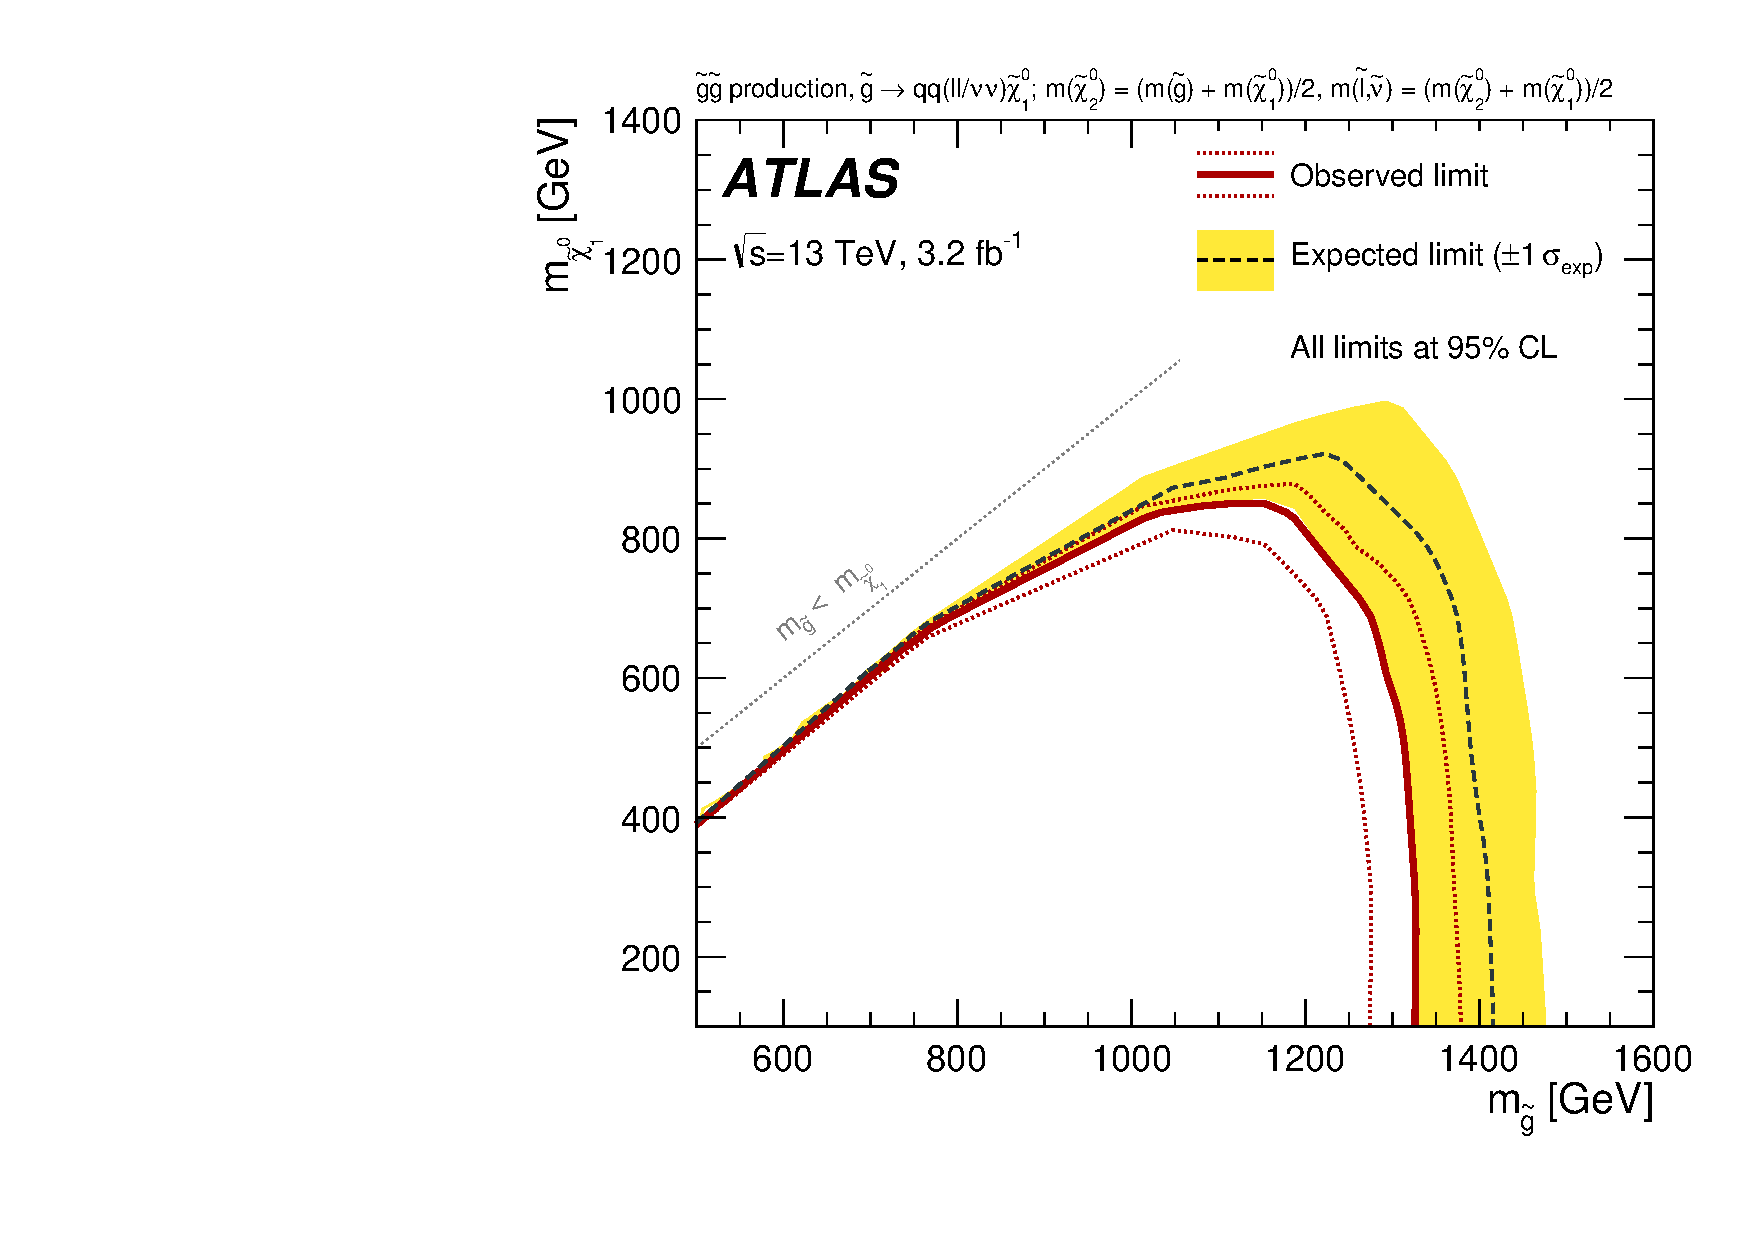
\includegraphics[width=0.49\textwidth]{PUB/FIGURES/exclusion2015SameSign_SR0b3j.pdf}}
\subfigure{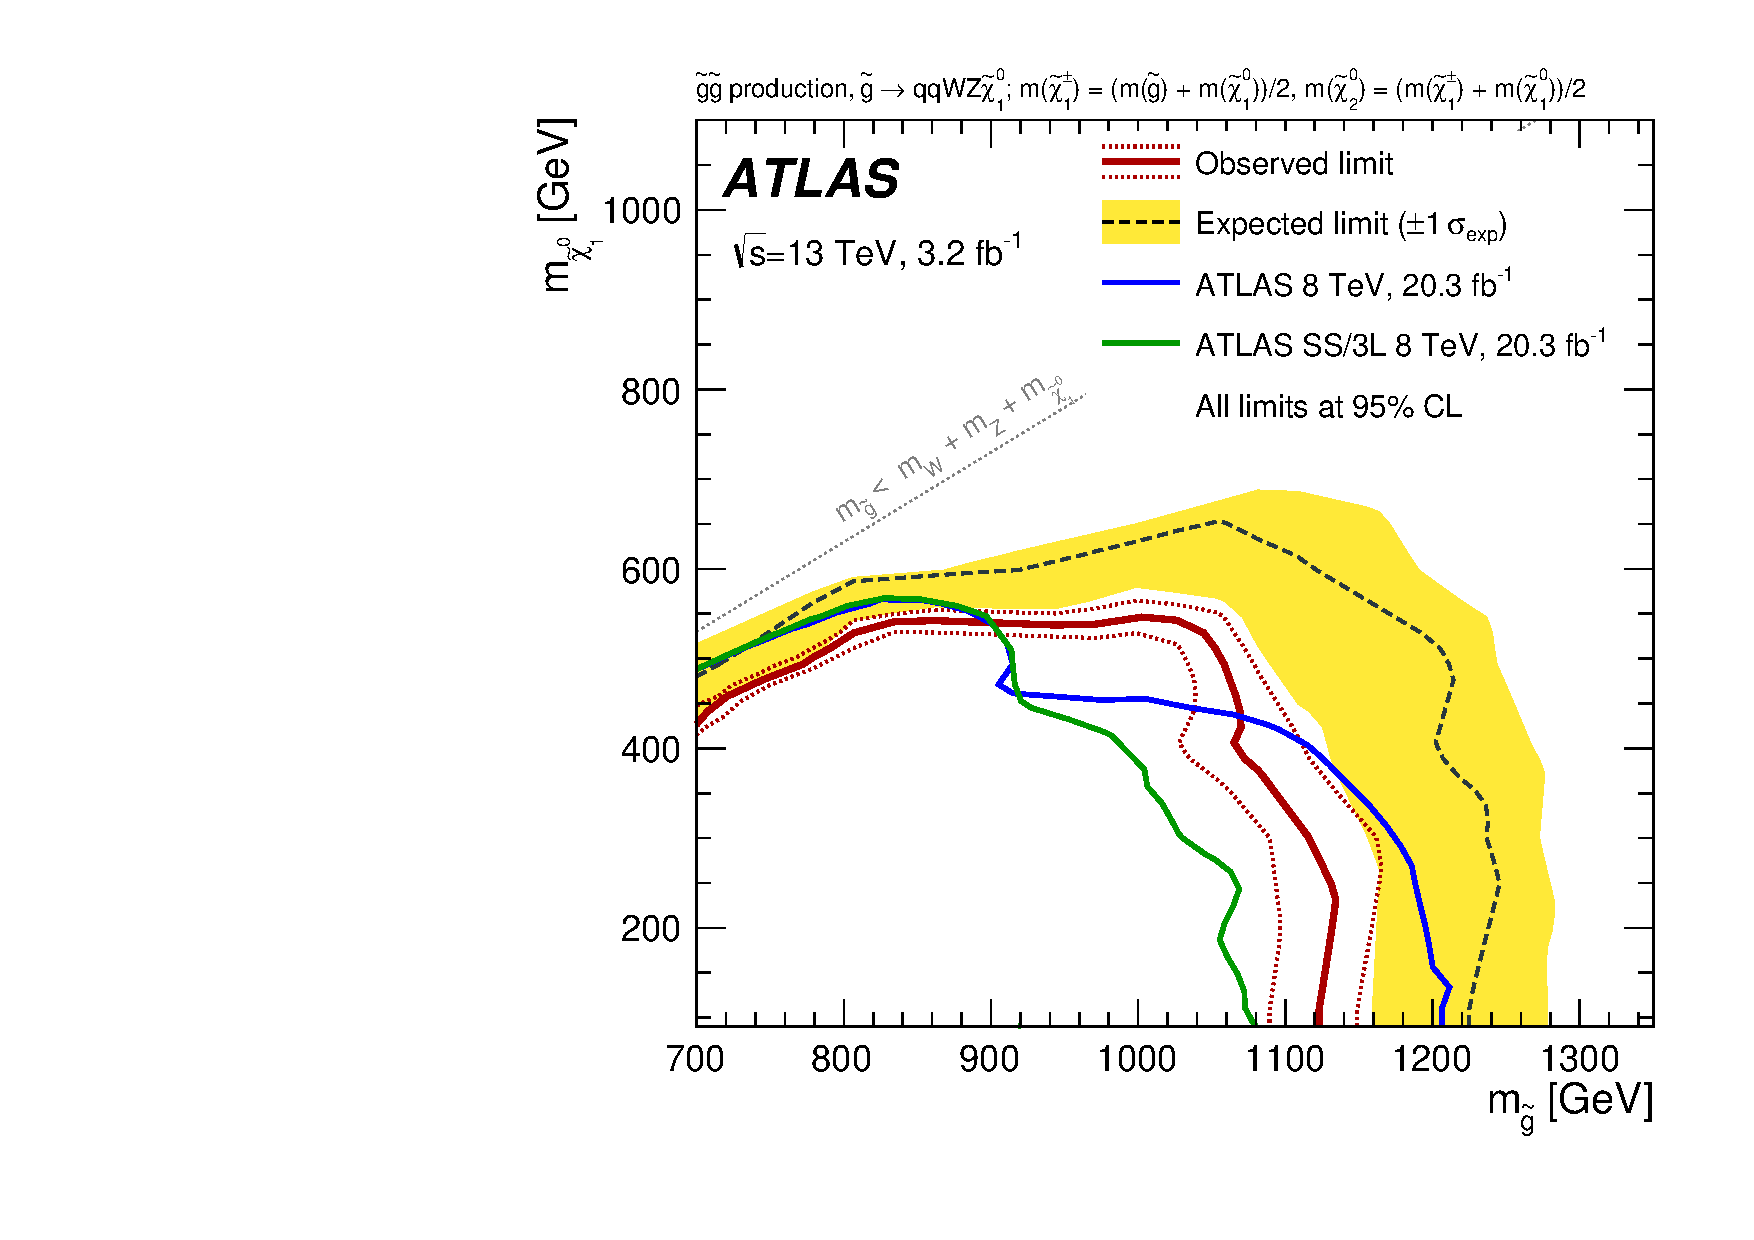
\includegraphics[width=0.49\textwidth]{PUB/FIGURES/exclusion2015SameSign_SR0b5j.pdf}}
\subfigure{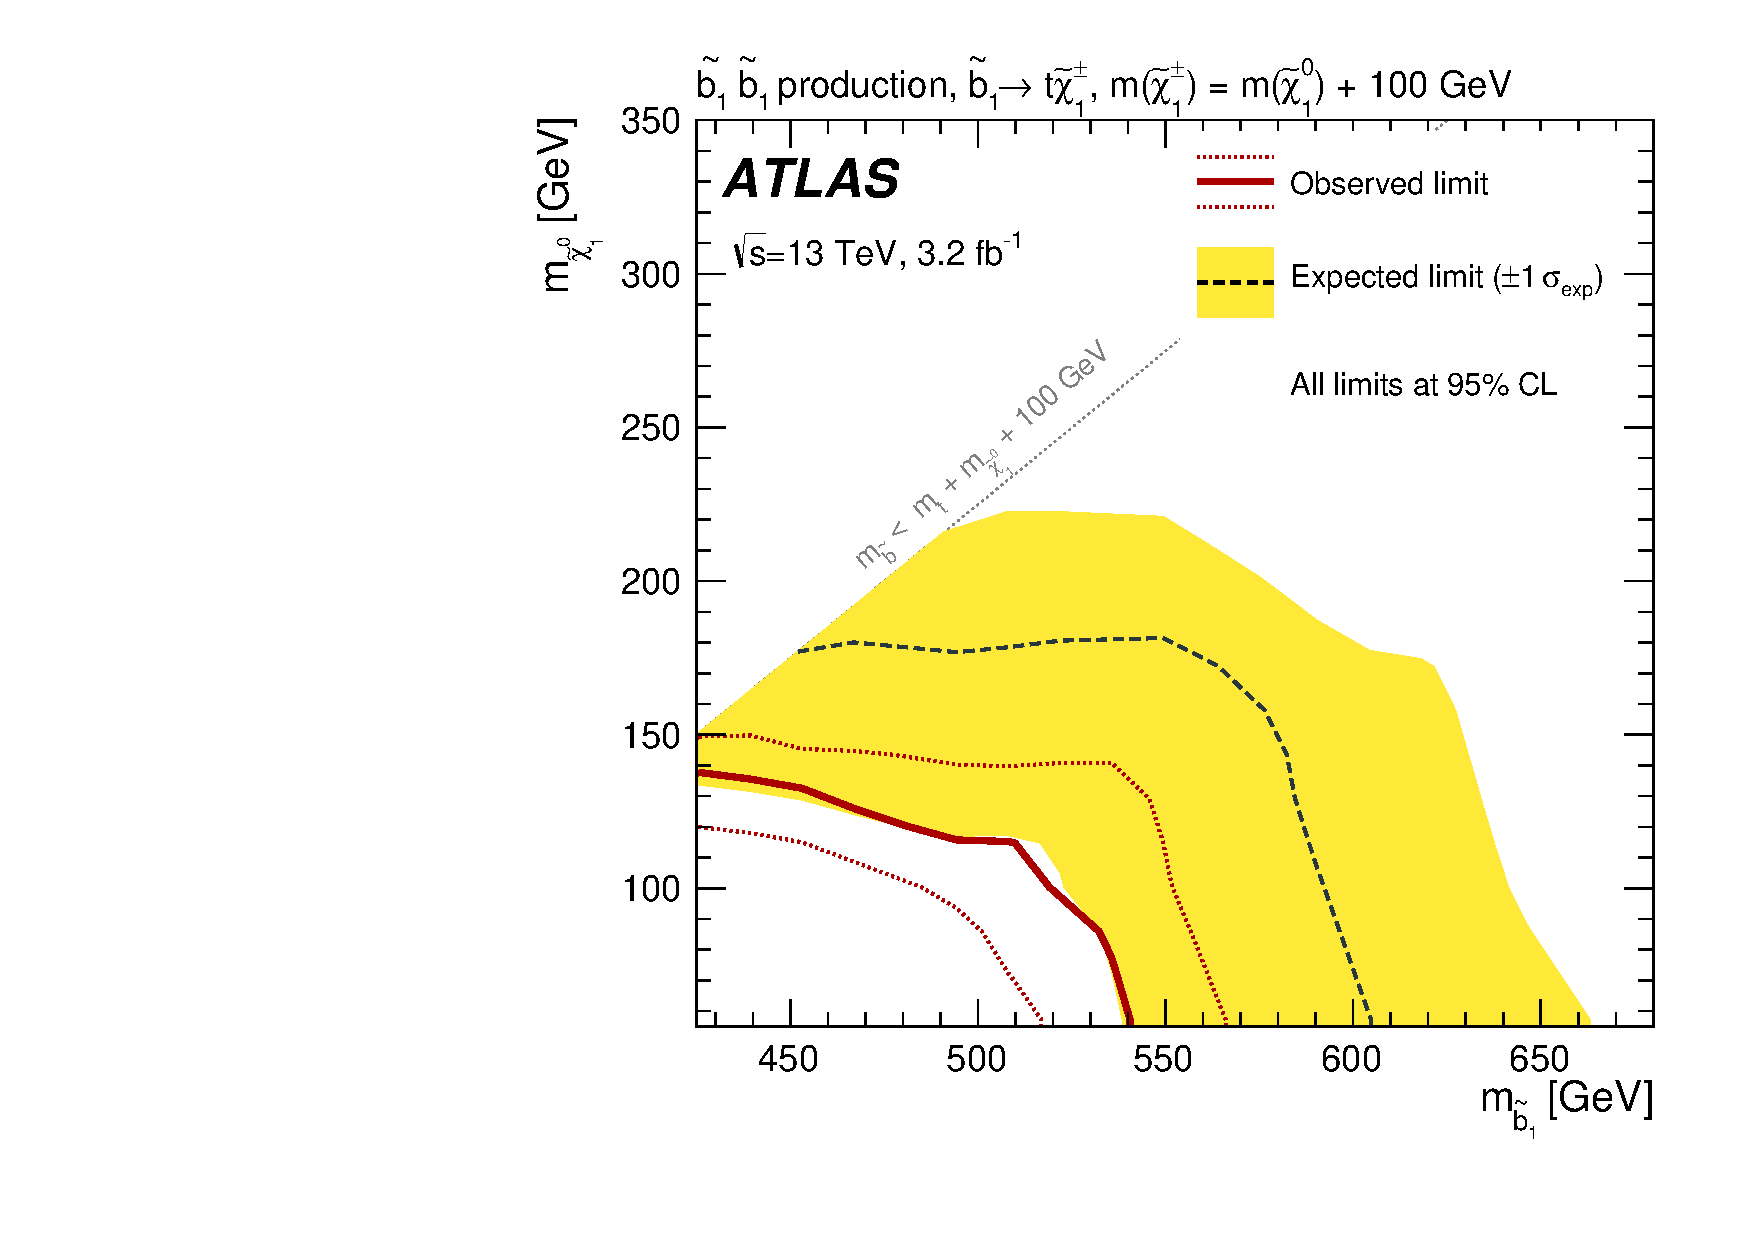
\includegraphics[width=0.49\textwidth]{PUB/FIGURES/exclusion2015SameSign_SR1b.pdf}}
\subfigure{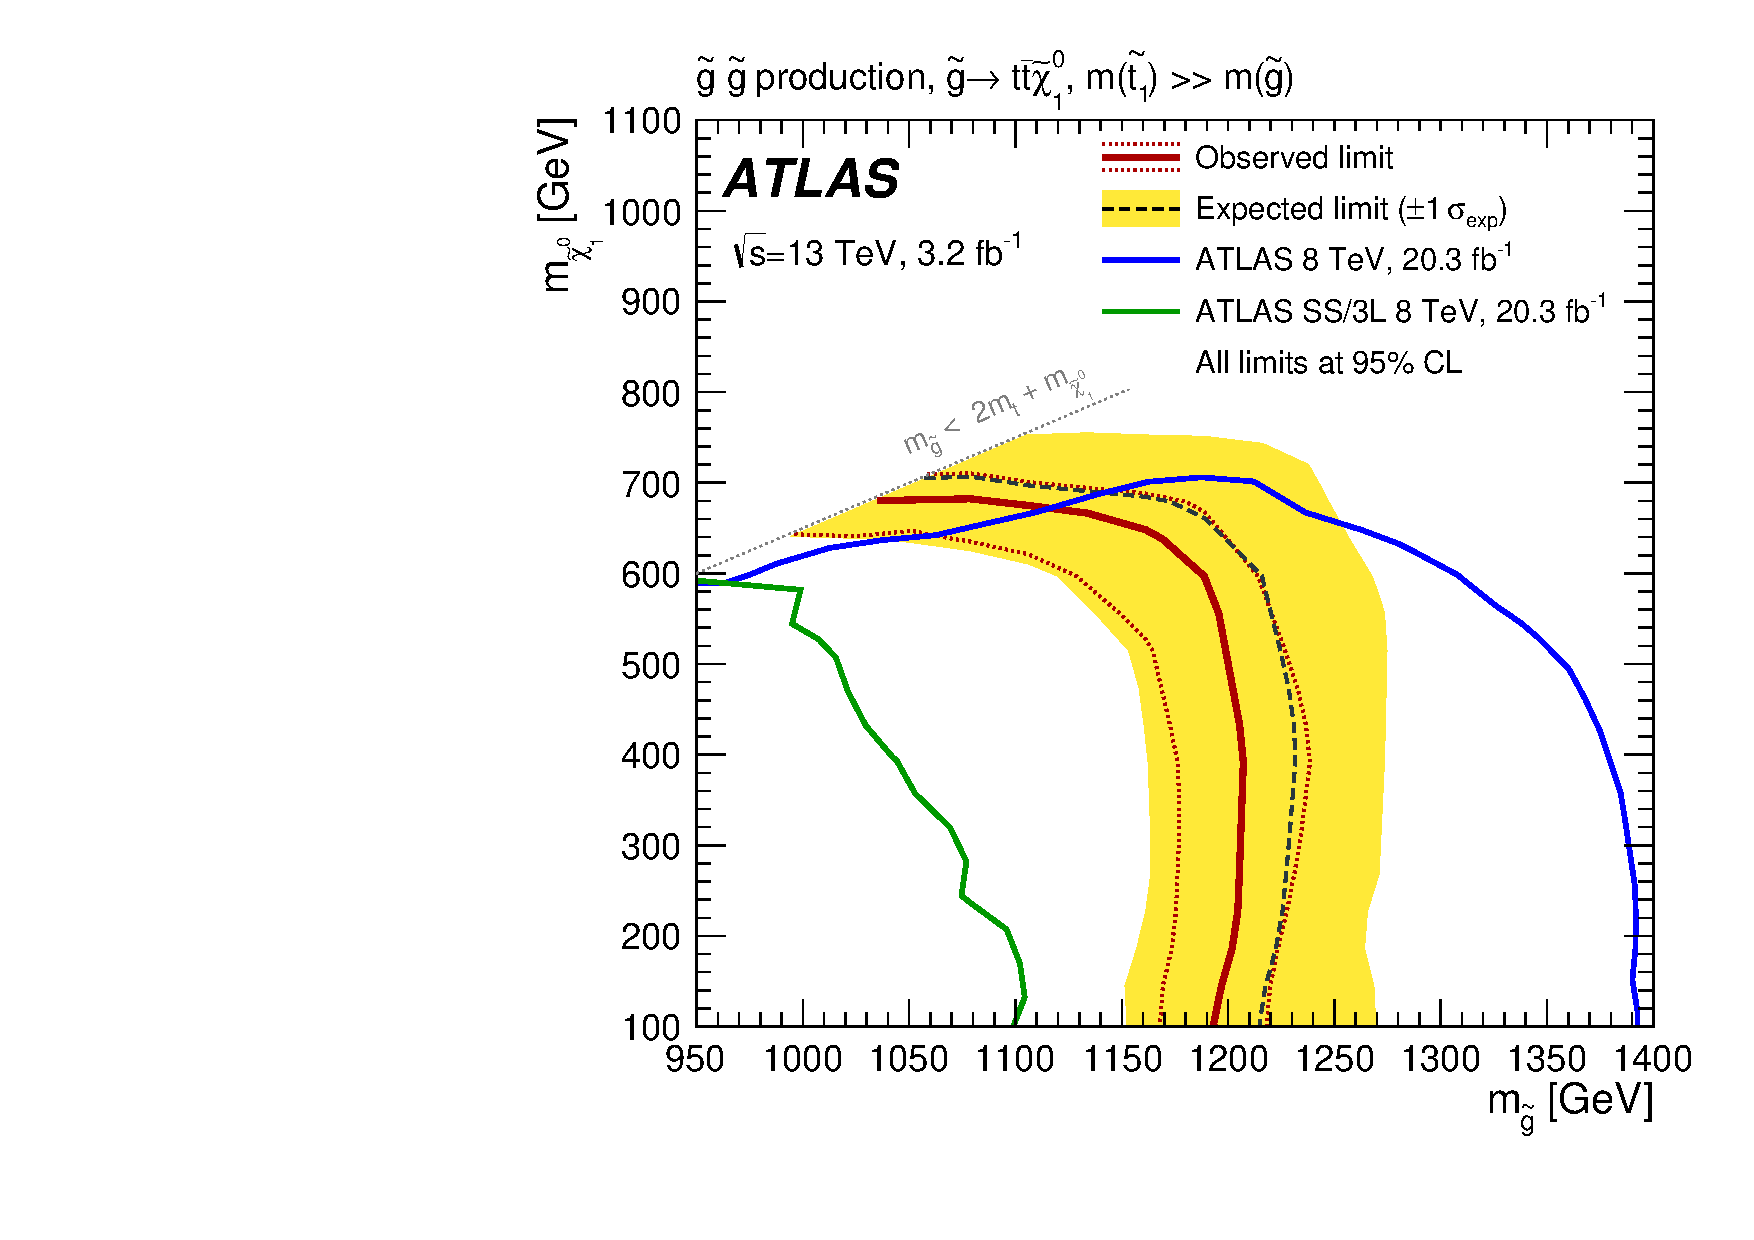
\includegraphics[width=0.49\textwidth]{PUB/FIGURES/exclusion2015SameSign_SR3b.pdf}}

\caption{Observed and expected exclusion limits on the \gluino, \sbottomone and \ninoone masses 
in the context of SUSY scenarios with simplified mass spectra 
featuring $\gluino\gluino$ or $\sbottomone \tilde{b}_{1}^{*}$ pair production with exclusive decay modes. 
The signal region used to obtain the limits is specified for each scenario. 
The contours of the band around the expected limit are the $\pm$1$\sigma$ results, 
  including all uncertainties except theoretical uncertainties on the signal cross-section. The dotted lines around the observed
    limit illustrate the change in the observed limit as the nominal signal cross-section is scaled up and down
    by the theoretical uncertainty. All limits are computed at 95\% CL.
Results are compared with the limits obtained by previous ATLAS searches
}
\label{fig:histfitter_final}
\end{figure}


%\label{fig:Results_SR_metD} 
%\end{figure} 
%
%
%\begin{figure}[htb!]
%\centering
%\subfigure{\includegraphics[width=0.49\textwidth]{HISTFITTER/{exclusion2015SameSignMc15SusyGtt_nom_IntNote_2.47fb_V02_Excl_winter2015SameSign_output_hypotest__1_harvest_fix_list}.pdf}}
%\subfigure{\includegraphics[width=0.49\textwidth]{HISTFITTER/{exclusion2015SameSignMc15SusyBtt_nom_IntNote_2.47fb_V02_Excl_winter2015SameSign_output_hypotest__1_harvest_fix_list}.pdf}}
%\subfigure{\includegraphics[width=0.49\textwidth]{HISTFITTER/{exclusion2015SameSignMc15SusyGG2StepWZ_nom_IntNote_2.47fb_V02_Excl_winter2015SameSign_output_hypotest__1_harvest_fix_list}.pdf}}
%\subfigure{\includegraphics[width=0.49\textwidth]{HISTFITTER/{exclusion2015SameSignMc15SusyGSL_nom_IntNote_2.47fb_V10_Excl_winter2015SameSign_output_hypotest__1_harvest_fix_list}.pdf}}
%
%\caption{Comparison of the analysis sensitivities for different signal grids.
%The exclusion curve obtained combining all the signal regions is only marginally
%better than the result obtained using only the best-berforming signal region. Data is blinded in this plot.}

The exclusion limits for the models of interest with their cross-section upper limits are shown in Figure~\ref{fig:Results_Limits_GN}.

\begin{figure}[htb!]
\centering
\subfigure{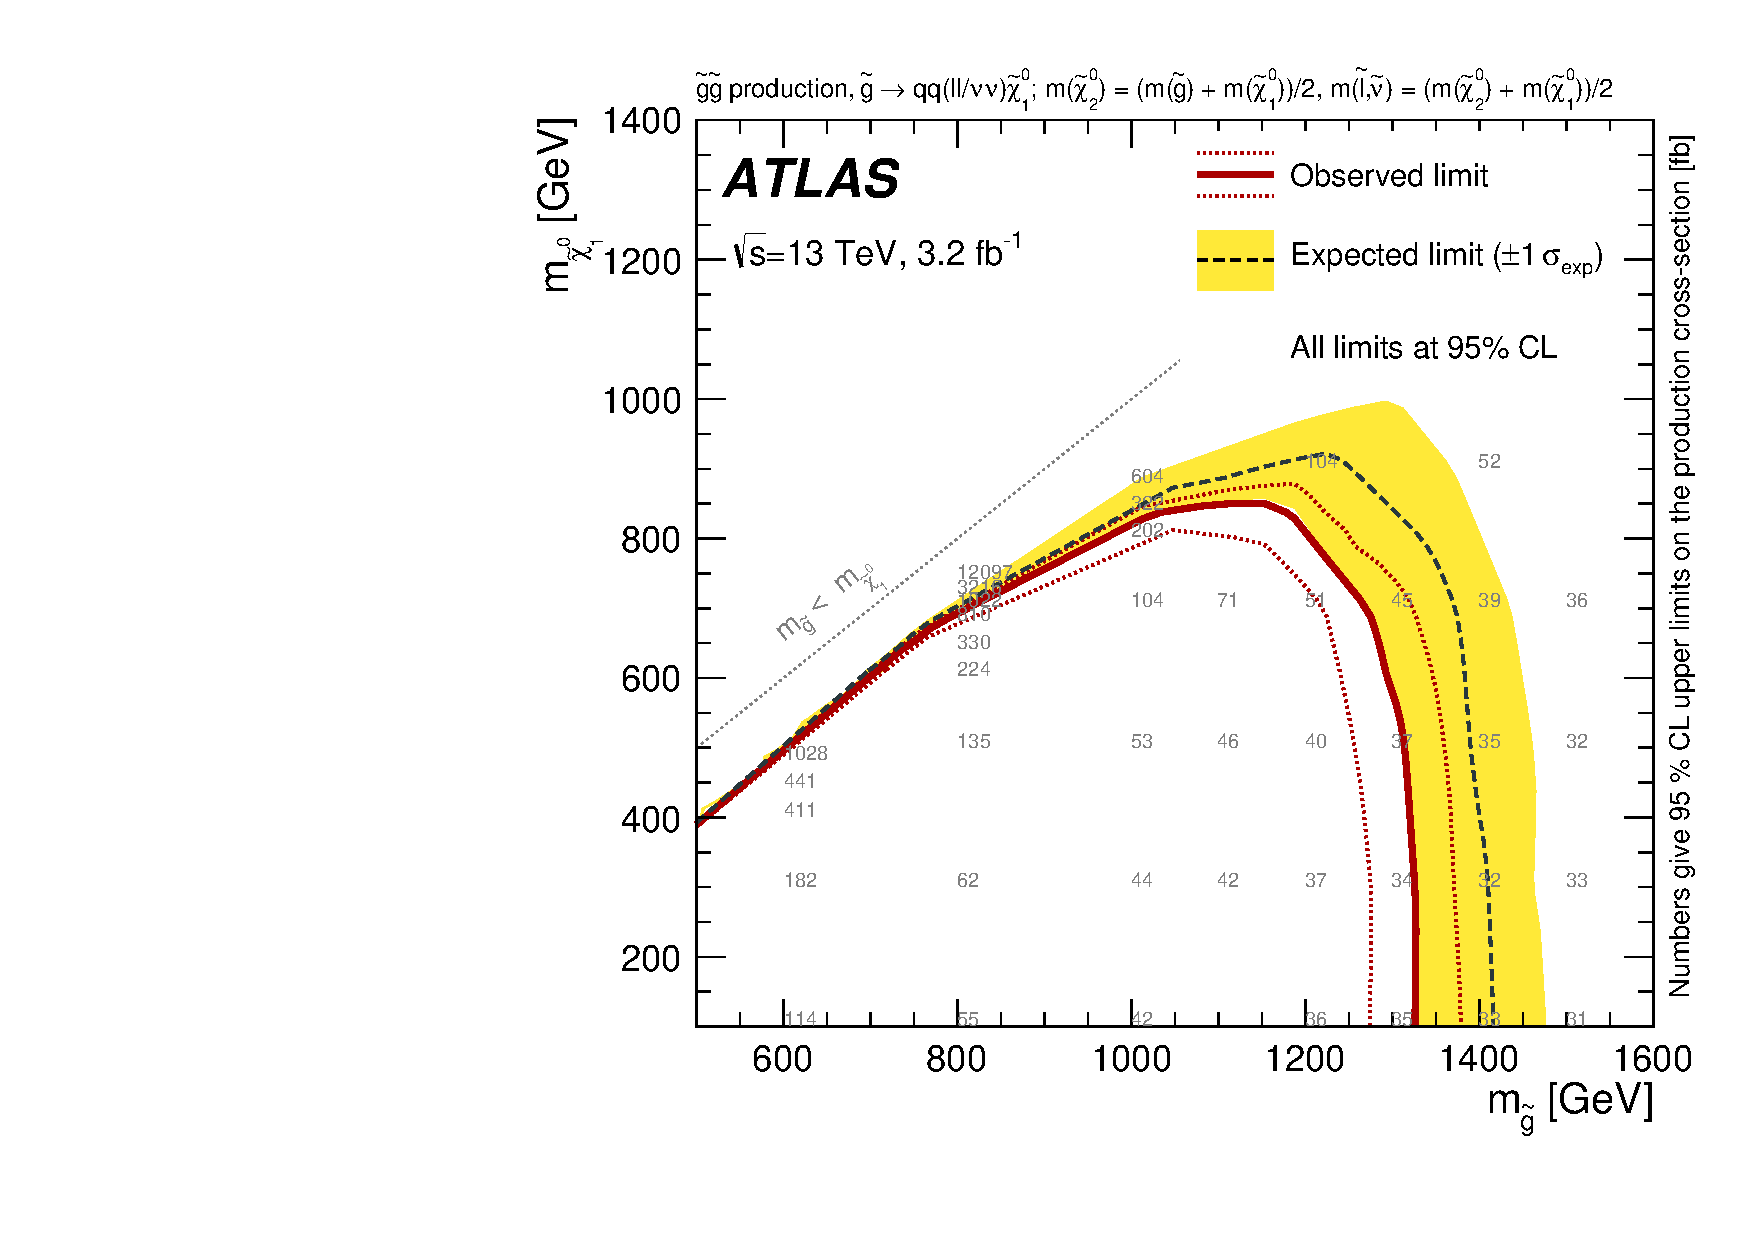
\includegraphics[width=0.48\textwidth]{PUB/FIGURES/exclusion2015SameSign_SR0b3jGN.pdf}}
\subfigure{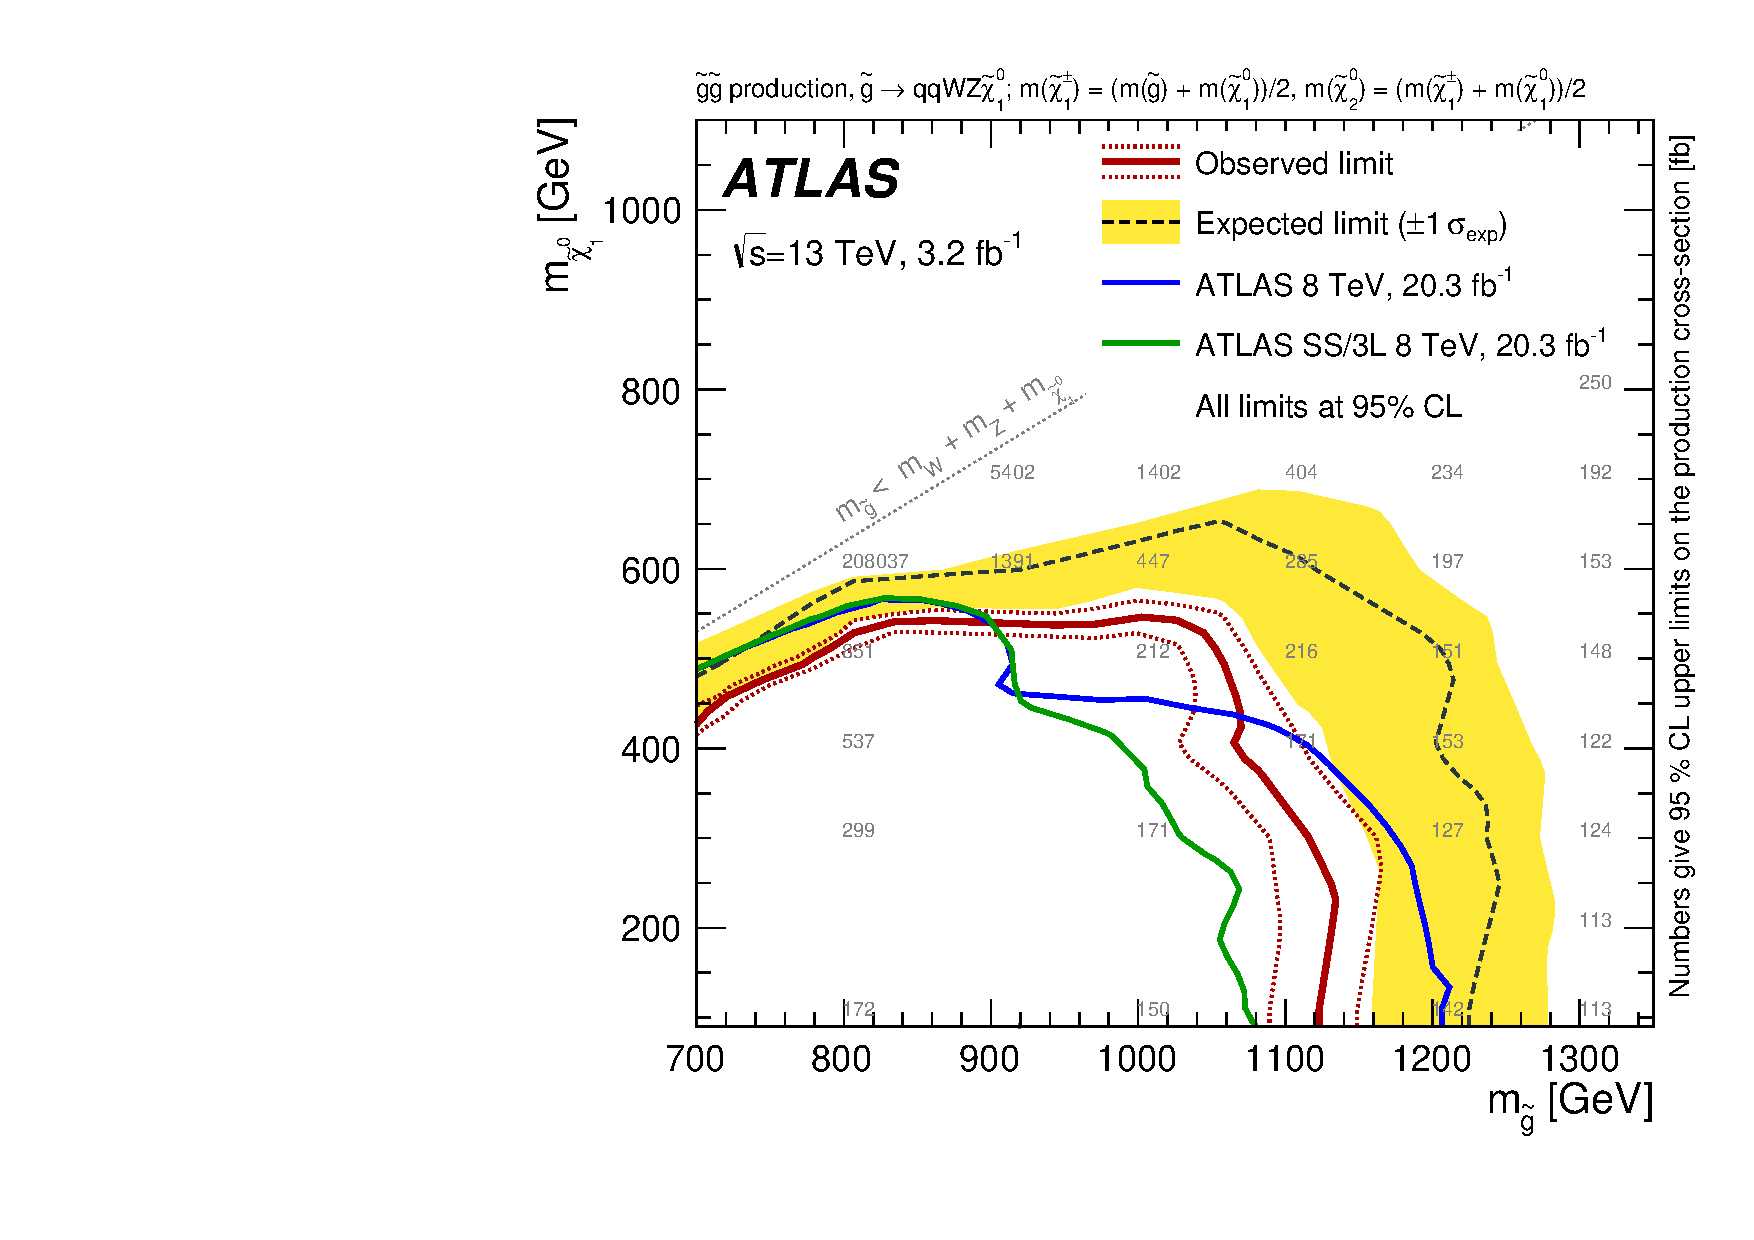
\includegraphics[width=0.48\textwidth]{PUB/FIGURES/exclusion2015SameSign_SR0b5jGN.pdf}}\\
\subfigure{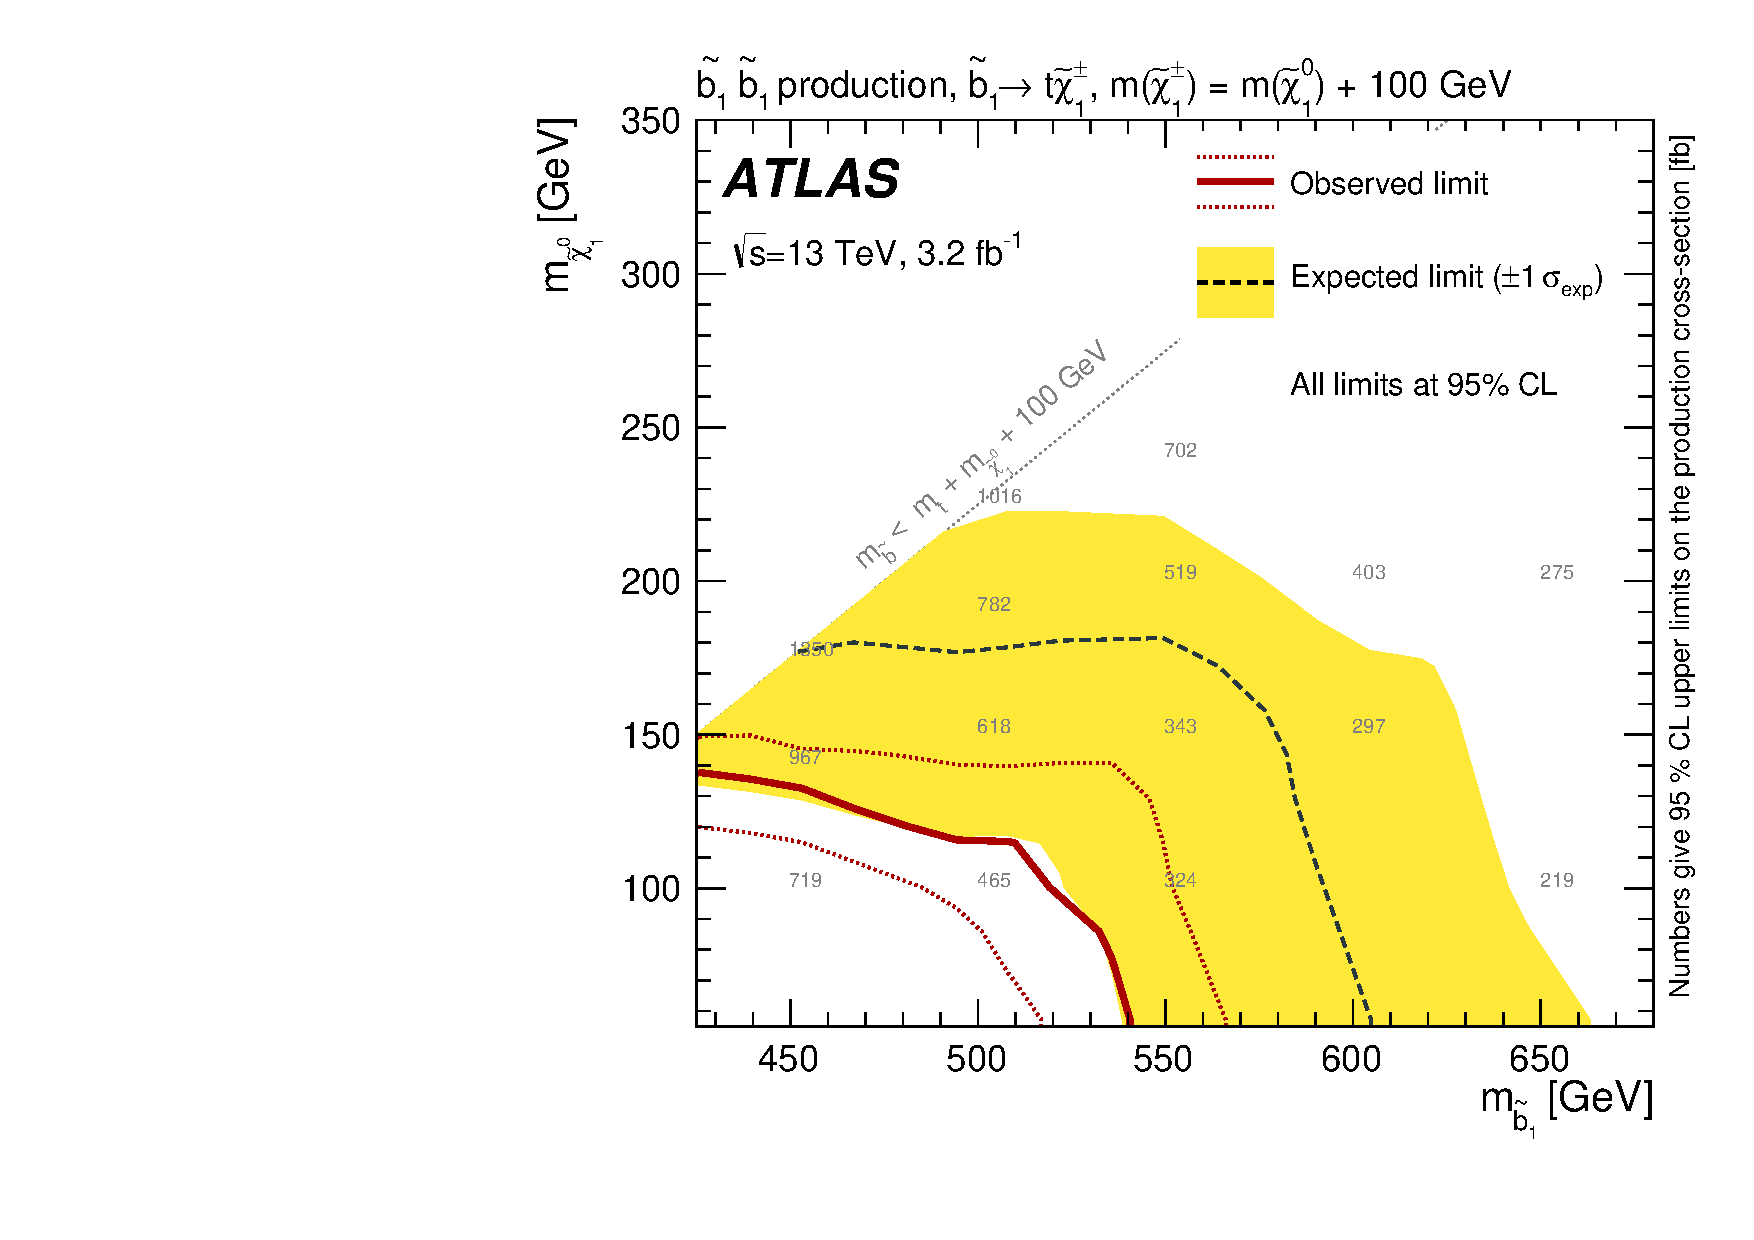
\includegraphics[width=0.48\textwidth]{PUB/FIGURES/exclusion2015SameSign_SR1bGN.pdf}}
\subfigure{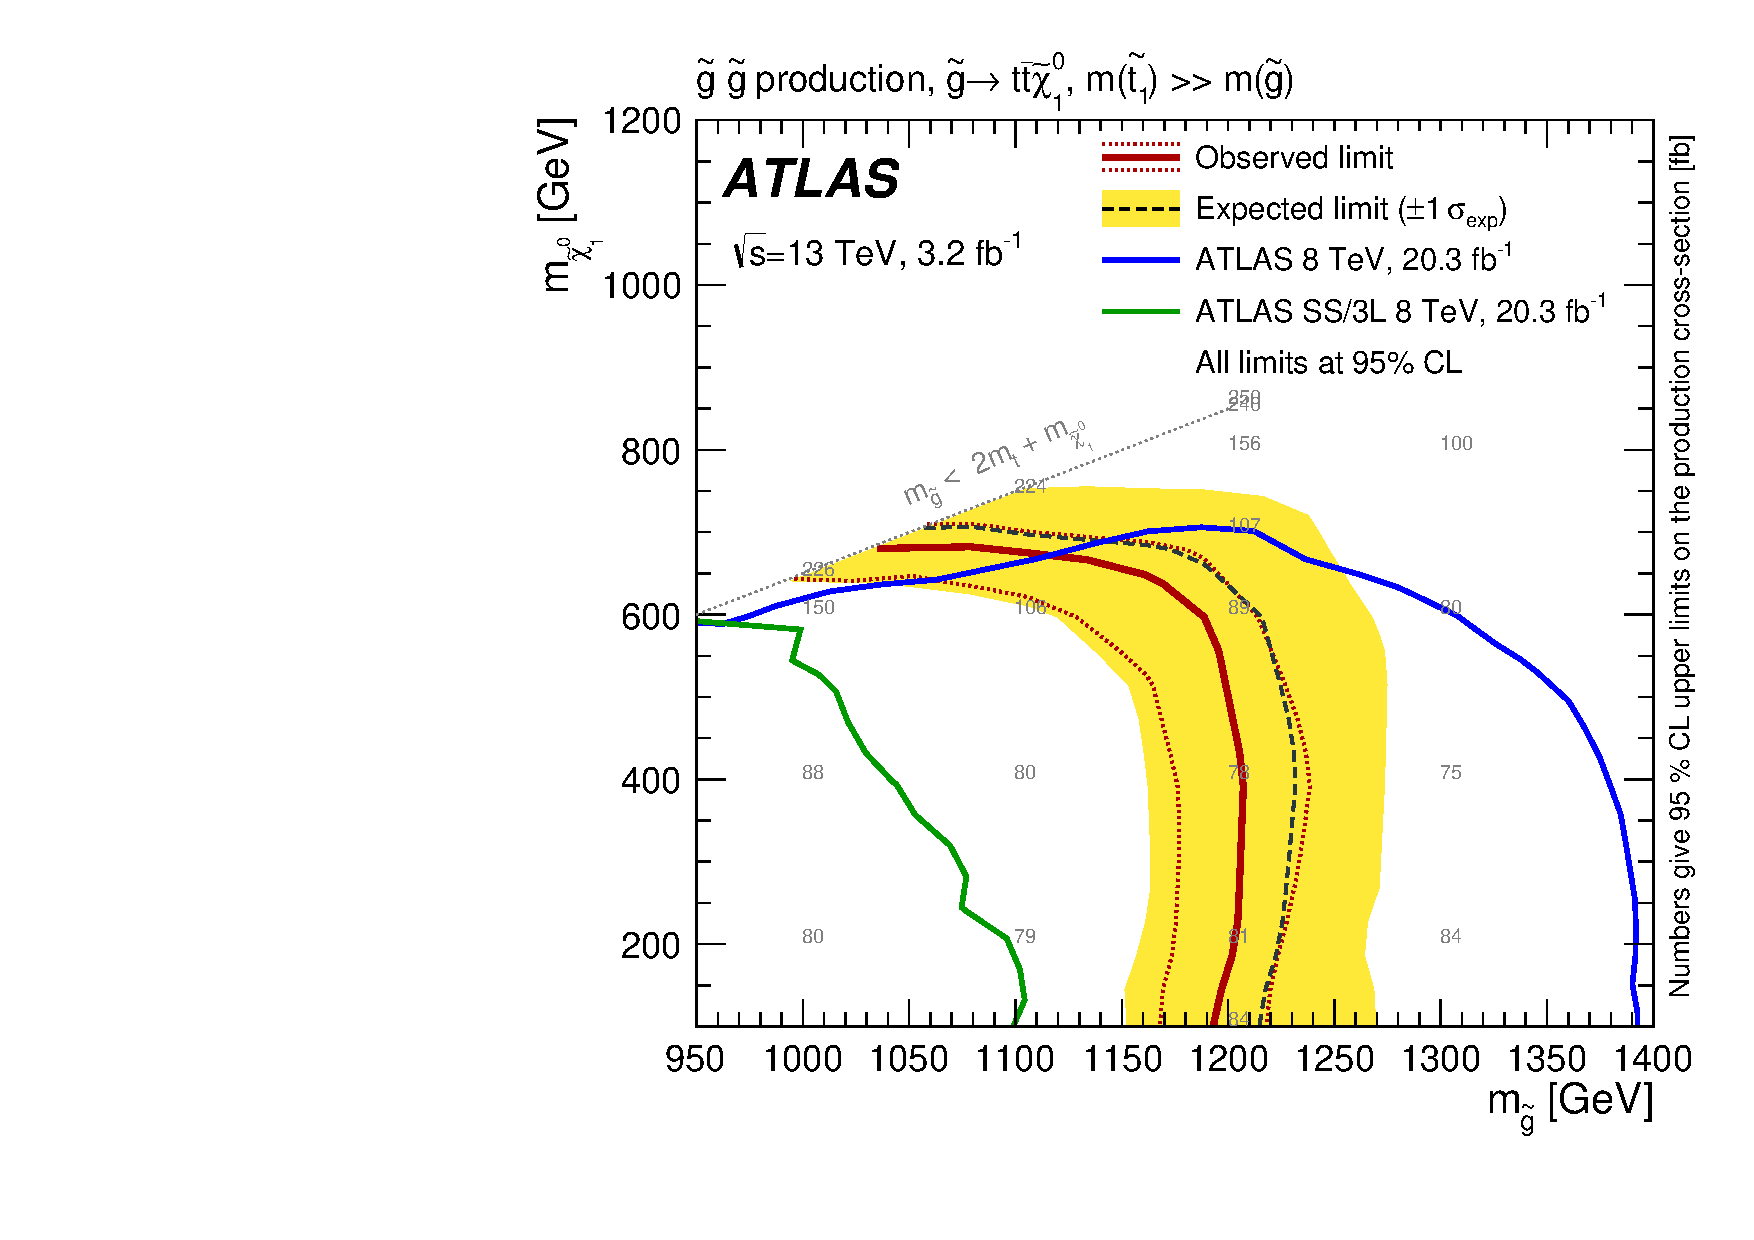
\includegraphics[width=0.48\textwidth]{PUB/FIGURES/exclusion2015SameSign_SR3bGN.pdf}}
\caption{Observed and expected exclusion limits on the \gluino, \sbottomone and \ninoone masses 
in the context of SUSY scenarios with simplified mass spectra 
featuring $\gluino\gluino$ or $\sbottomone \tilde{b}_{1}^{*}$ pair production with exclusive decay modes. 
The contours of the band around the expected limit are the $\pm$1$\sigma$ results, 
  including all uncertainties except theoretical uncertainties on the signal cross-section. The dotted lines around the observed
    limit illustrate the change in the observed limit as the nominal signal cross-section is scaled up and down
    by the theoretical uncertainty. All limits are computed at 95\% CL.
The grey numbers show 95\% CL upper limits on cross-sections (in fb) obtained using the signal efficiency and acceptance specific to each model.}
\label{fig:Results_Limits_GN} 
\end{figure}
